\subsection{Analytical Jacobian in the Singular Regime}

Figure \ref{fig:singular-epsilon-analytic} presents the singular epsilon stress test utilizing an analytically derived Jacobian for LSODA and CVODE. For LSODA, the exact derivative yields no structural improvement. The failure boundaries remain identical to the numerical baseline, collapsing at highly singular indices (\(p \le 1.10\)) when \(\varepsilon \le 10^{-12}\). In the surviving \(p = 1.25\) case, the analytical Jacobian provides only a execution time reduction (e.g., 40.7 seconds at \(\varepsilon = 10^{-30}\) instead of 46.3), confirming that LSODA's failures stem from algorithmic limits rather than finite-difference inaccuracies.

CVODE exhibits a distinct behavioral shift. While it continues to fail at intermediate regularization values (e.g., \(\varepsilon = 10^{-12}\) and \(10^{-14}\) at \(p = 1.25\) and \(p = 1.01\)), the analytical Jacobian unexpectedly rescues the integration at the absolute extreme limit of \(\varepsilon = 10^{-30}\). Under these conditions, CVODE resolves the physics in 0.16 seconds and 0.10 seconds respectively. This demonstrates that while the analytical Jacobian introduces detrimental overhead in degenerate regimes for CVODE, it fixes the extreme finite-difference conditioning errors present in strongly singular limits.

\begin{figure}[H]
  \centering
  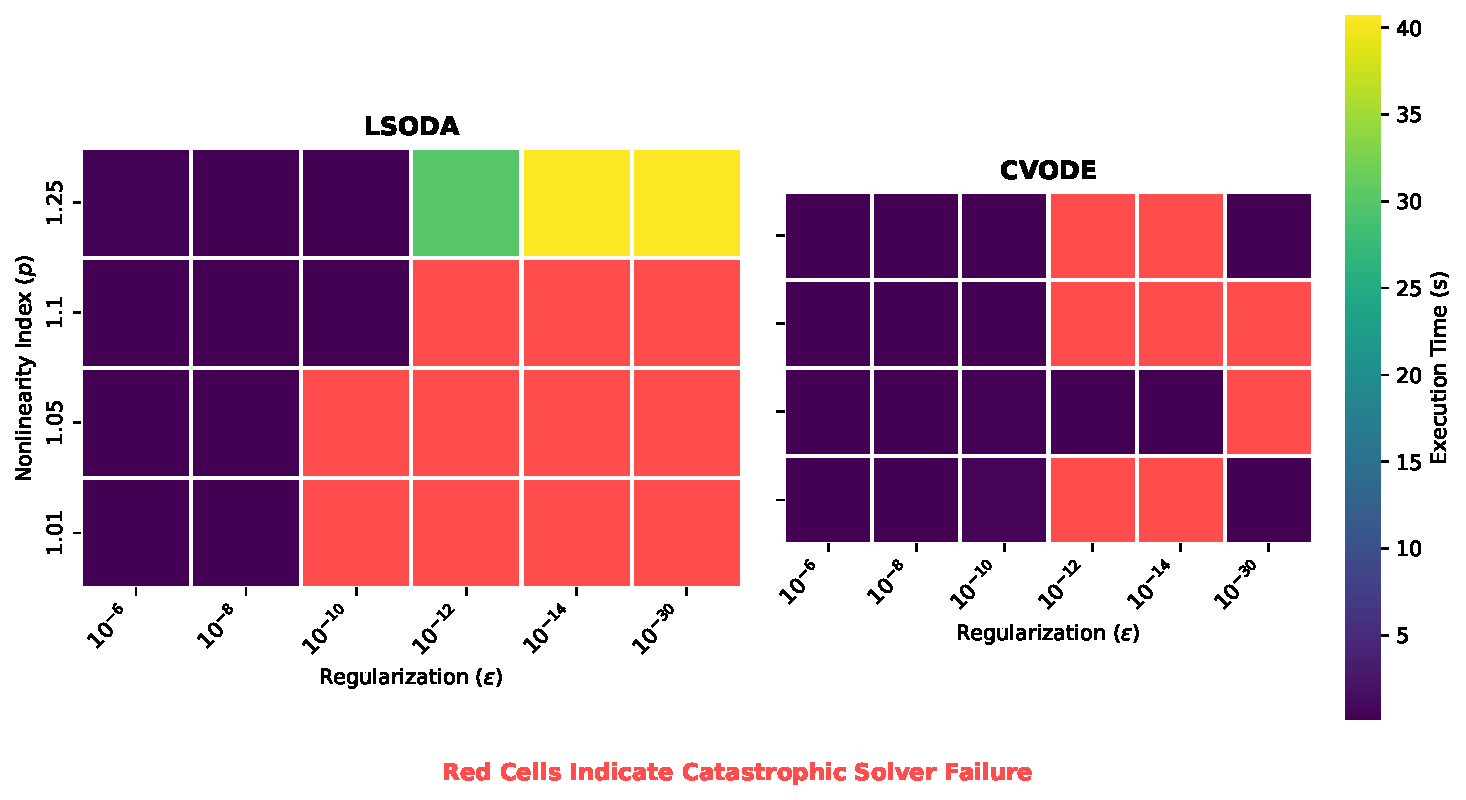
\includegraphics[width=\textwidth]{images/stability_matrix_lsoda_cvode_analytic.pdf}
  \caption{Execution times and failure boundaries for LSODA and CVODE utilizing an analytical Jacobian.}
  \label{fig:singular-epsilon-analytic}
\end{figure}
